% THIS IS SIGPROC-SP.TEX - VERSION 3.1
% WORKS WITH V3.2SP OF ACM_PROC_ARTICLE-SP.CLS
% APRIL 2009
%
% It is an example file showing how to use the 'acm_proc_article-sp.cls' V3.2SP
% LaTeX2e document class file for Conference Proceedings submissions.
% ----------------------------------------------------------------------------------------------------------------
% This .tex file (and associated .cls V3.2SP) *DOES NOT* produce:
%       1) The Permission Statement
%       2) The Conference (location) Info information
%       3) The Copyright Line with ACM data
%       4) Page numbering
% ---------------------------------------------------------------------------------------------------------------
% It is an example which *does* use the .bib file (from which the .bbl file
% is produced).
% REMEMBER HOWEVER: After having produced the .bbl file,
% and prior to final submission,
% you need to 'insert'  your .bbl file into your source .tex file so as to provide
% ONE 'self-contained' source file.
%
% Questions regarding SIGS should be sent to
% Adrienne Griscti ---> griscti@acm.org
%
% Questions/suggestions regarding the guidelines, .tex and .cls files, etc. to
% Gerald Murray ---> murray@hq.acm.org
%
% For tracking purposes - this is V3.1SP - APRIL 2009

\documentclass{sig-alternate-10pt}
\pdfpagewidth=8.5in
\pdfpageheight=11in

\usepackage{array}
%\usepackage[tight,footnotesize]{subfigure}
\usepackage{subcaption}
\usepackage{multirow}
%\usepackage{graphicx}
%\usepackage{framed}
\usepackage{balance}
\usepackage{url}
%\usepackage{amsmath}
\usepackage{float}
\usepackage{enumerate}
\usepackage{cite}

%\usepackage{lipsum}

\graphicspath{{figures/}}

\newcommand{\ignore}[1]{
  % Use to comment out large blocks of text
}

%\makeatletter
%\def\@copyrightspace{\relax}
%\makeatother

\begin{document}

\title{Searching for the Higgs Boson Particle \\ using Data Analytics}


\numberofauthors{3}

\author{
%
\alignauthor
Ananya Choudhury\titlenote{Ananya worked on shallow and deep learning techniques.}\\
       \affaddr{Dept. of Computer Science}\\
       \affaddr{Virginia Tech}\\
       \affaddr{Blacksburg, U.S.A}\\
       \email{ananya@vt.edu}
%
\alignauthor
Vivek Bharath Akupatni\titlenote{Vivek worked on Bayesian classifiers, tree-based classifiers, and function-based classifiers.}\\
       \affaddr{Dept. of Computer Science}\\
       \affaddr{Virginia Tech}\\
       \affaddr{Blacksburg, U.S.A}\\
       \email{vivekb88@vt.edu}
%
\alignauthor 
Vignesh Adhinarayanan\titlenote{Vignesh worked on instance-based classifiers and ensemble methods. \\All authors contributed to the writing of their respective parts. The authors freely exchanged ideas with each other regardless of the primary focus of their work.}\\
       \affaddr{Dept. of Computer Science}\\
       \affaddr{Virginia Tech}\\
       \affaddr{Blacksburg, U.S.A}\\
       \email{avignesh@vt.edu}
}

\maketitle

\begin{abstract}

Abstract goes here

\end{abstract}

\section{Introduction}
\label{sec:introduction}

Introduction goes here

%\begin{figure}[h]
%\centering
%\includegraphics[width=1.0\columnwidth]{accelerators-top500}
%\caption{Number of Systems Using Accelerators in the Green500 Lists.}
%\label{fig:green500-trends}
%\end{figure}


\section{Background}
\label{sec:background}

The LHC collides bunches of proton every 50 ns producing a random number of proton-proton collisions called events. These events produce new particles, most of which are very unstable and decays quickly. The ATLAS detector measures three properties of these surviving particles: type, energy and 3D direction of the particle. Based on these properties,  the property of the heaviest primary particles is inferred. An online trigger system selects about 400 events per second producing 3 pb of raw data per year.

Each event contains about ten particles of interest in the final state. The particles of interest for this challenge are electrons, muons, hadronic tau, jets and missing transverse energy. Electrons and muons live longer enough to reach the detector, so their properties (direction and energy) can be measured directly. The other particles such as tau, hadron and jets decays into different particles and hence their properties are inferred using the law of momentum conservation.  The measured momenta of all the particles of the event is the primary information provided in the dataset. 

Higgs boson is a particle which is responsible for the mass of the other elementary particles. In the original discovery, the Higgs boson was seen decaying into $\gamma\gamma$, WW, and ZZ, which are all boson pairs~\cite{Ananya1,Ananya2} . The signal class comprises of events in which Higgs boson decays into two taus. Our goal is to identify those signals from a significantly higher number of background events.

\section{Related Work}
\label{sec:related}

Detecting exotic particles in high-energy physics (HEP) using data analytics techniques instead of the traditionally used physical detectors~\cite{detectors} is not new. Cutts et al. are among the first to use neural networks to identify interesting events in HEP experiments~\cite{Cutts-NN1}. This was quickly followed by several attempts in improving the classification accuracy of neural networks~\cite{NN2,NN3}. Apart from the widely popular techniques based on neural networks, only decision trees were explored for a long time. Bowser-Chao and Dzialo used binary decision trees wto detect top quarks and compared their results with neural networks~\cite{Binary-DT}. The conventional wisdom was that neural networks were by far the best when it comes to classification in HEP until Roe et al. came along and projected boosted decision trees as an alternative to artificial neural networks~\cite{Boosted-DT}. By combining several \emph{weak} classifiers, Roe et al. showed that it is possible to obtain better accuracy than a neural network. However, more recently, Baldi et al. showed that a deep learning neural network with several hidden layers outperforms the boosted decision tree~\cite{DeepNN}. While a number of classification techniques have been developed and applied over the last several years, the HEP community has so far explored only neural networks and boosted decision trees in any depth. This lead to the development of statistical packages for the HEP community such as StatPatternRecognition so that several other techniques based on Rotation Forest, Discriminant Analysis etc. could be explored~\cite{StatPatternRecognition}. Despite this effort, no documented work exists in HEP where alternative techniques are explored even though other techniques are thought to be inferior.

Since Baldi et al.~\cite{DeepNN} work is closest to ours, we describe it in detail here. The authors in this paper used deep learning methods of neural network to find exotic particles in high energy particle colliders. Deep learning models are neural networks with multiple hidden networks. Current technics like shallow models which are single hidden layer feedforward network fail to capture all features.
The deep learning model here is used on 2.6 million training examples and 100,000 validation examples. The mode is a five-layer neural network with 300 hidden units in each layer, learning rate of 0.05, and a weight decay coefficient of 0.00001 . Testing is done on 500,000 examples. For Higgs benchmark, Area Under the Curve(AUC) - complete for deep neural network is 0.88 and for shallow neural network = 0.81.

\section{Methodology}
\label{sec:methodology}


\subsection{Data Preprocessing}
In some situations, it becomes difficult to measure the physical properties of a particle such as momentum and energy accurately. In our original dataset, as many as 177000 out of 250000 instances had missing attributes. We considered three approaches to deal with missing values. First, we tried ignoring instances with missing attributes. But this resulted in very few useful instances. Second, we tried to replace the missing values with the mean/median. However, this biases the experiments. Finally, we decided to adopt a method known as multiple imputations~\cite{MultipleImputation} which replaces the missing values with a random number that follows the distribution for that attribute. We use the \texttt{Amelia}~\cite{Amelia} package to perform this task.



\subsection{Feature Engineering and Selection}

\begin{figure*}[t]
\centering
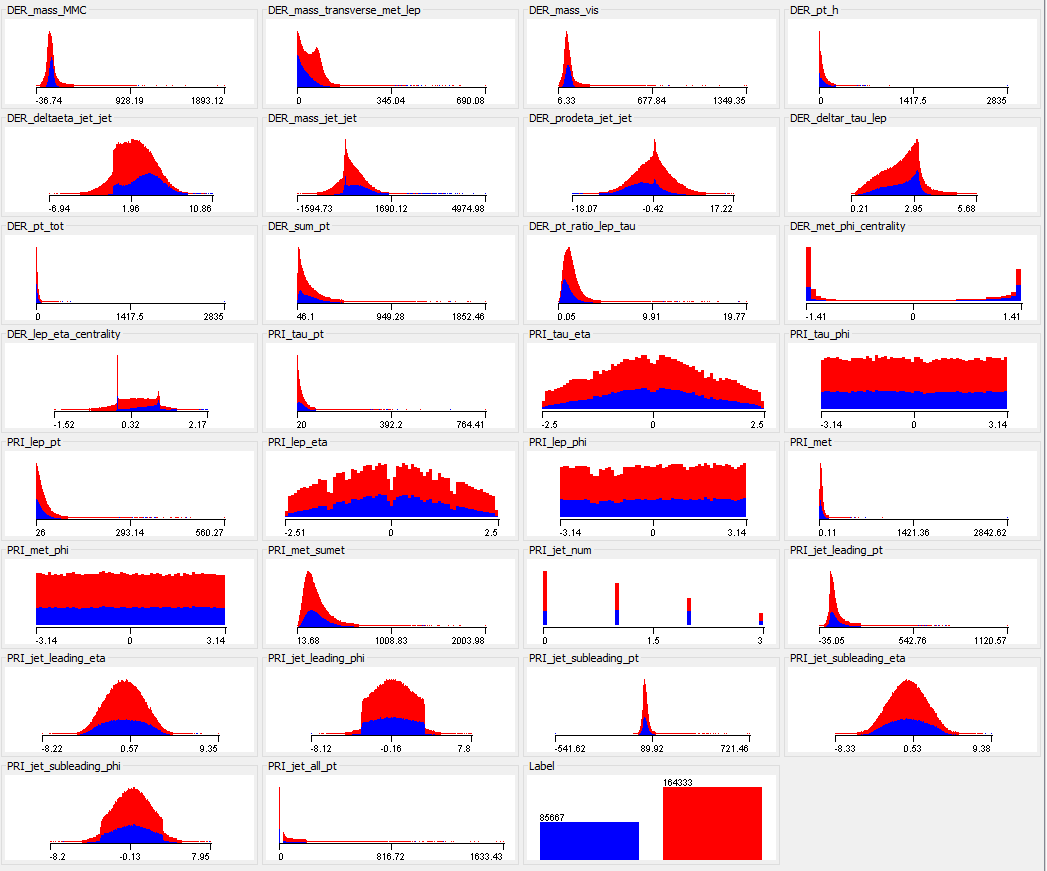
\includegraphics[width=1.8\columnwidth]{Distribution}
\caption{Distribution of different attributes for signal. Blue represents signal and red represents background.}
\label{fig:distribution}
\end{figure*}

The raw dataset includes 17 features. From these 17 basic features, 13 additional features were derived. These 13 derived features describe some property of the particle and requires knowledge of physics. The features are provided by physics. Their description is given in the appendix. From these 30 features, a subset is selected based on the following factors. First, we decide the ability of the feature/attribute to distinguish between signal an background. The distribution of different attributes is shown in Fig.~\ref{fig:distribution} for signal and background separately. Second, we try to avoid using features correlating with each other while building the classifier. Fig.~\ref{fig:correlation-matrix} shows the correlation matrix of the features. The final set of features selected differs for each classifier. The details are given in their respective subsections.

\begin{figure}[h]
\centering
\includegraphics[width=1.0\columnwidth]{corr}
\caption{Correlation matrix. Dark blue indicates features that shows strong positive correlation. Dark red indicates features that show strong negative correlation.}
\label{fig:correlation-matrix}
\end{figure}



\subsection{Data Analytics Techniques}

In this section, we describe the various classification schemes we explored. For each technique, we also describe the parameter settings explored in brief.


\subsubsection{Bayesian Classifiers}

\paragraph{Naive Bayes}

This classifier is based on the Naive Bayes technique developed by John et al.~\cite{NaiveBayes}. The modeling and prediction overhead were negligible as this method is known to be highly scalable. This method could classify background noise better when compared to signal. During data preprocessing step, we included only those features whose Pearson correlation coefficient was below a particular threshold. Our experiments suggested that out by increasing the threshold value, which in turn increases of number of correlated features, resulted in decrease in the performance of this method.The best performance is achieved when the dataset included 12 features whose pairwise correlation coefficient is less than 0.6.	

\subsubsection{Functions-based Classifiers}

\paragraph{Logistic Regression}

This classifier is based on the Ridge estimation technique developed by Cessie et al.~\cite{Logistic Regression}. Being a linear method, the modeling and prediction overhead were small. In this technique, we used L1 regularized logistic regression. We explored the performance of this method
by varying the number of features in the dataset. The results on our dataset suggest that performance seems to be more or less the same with varying number of features.

\paragraph{Linear Discriminant Analysis}

This linear classifier fits a gaussian distribution of equal variance to each of the classes. We took the class priors to be equal when evaluating this method. The results on our dataset indicate that performance of this technique remains more or less the same when number of features are varied.

\paragraph{Quadratic Discriminant Analysis}

This linear method is similar to Linear Discriminant Analysis, expect that this technique uses quadratic decision boundaries. In evaluating this method, we used equal class priors. The optimal performance shown in the table is obtained when the dataset included features whose pairwise correlational coefficient is less than 0.95.

\subsubsection{Tree-based Classifiers}

\paragraph{Decision Tree Classifier}

In evaluating the performance of decision tree classifier, we used "gini" and "entropy" criterion.These two criterion on our dataset produced similar results. We varied the minimum number of samples required to split an internal node, and the best performance was achieved when this value was 300.  The optimal results for this classifier are shown in the table.

\subsubsection{Instance-based Classifiers}

\paragraph{k-Nearest Neighbor}

For the instance-based classifier we explore the k-nearest neighbor (kNN) technique~\cite{kNN}. This is a lazy classification technique in which the \emph{k} nearest neighbors are looked at to decide the class of a new instance. This technique has practically no training overhead. The classification overhead is very high though, particularly if the distance for all previously seen instances are computed exhaustively. Since this technique is known to perform bad with noisy attributes and irrelevant attributes, we explore removing such attributes from our dataset. We also tried to construct the classifier using top few principal components in order to keep only relevant features. In addition, we also experiment with the number of neighbors considered.


\subsubsection{Neural Networks}

For Higgs Boson project, we used both deep and shallow neural networks. We analyzed our data using multiple networks each of which are discussed below. 


\paragraph{feedforwardnet} Feed Forward networks consist of a series of layers. The first layer has a connection from the network input. Each subsequent layer has a connection from the previous layer. The final layer is the output layer which produces the network output. 
The hidden layer is of size 60. The transfer function used in this layer is 'tansig' (tan-Sigmoid Transfer Function). Tansig is a neural network transfer function which calculates a layer's output from its net input. The output layer produces only 1 output ( 0 or 1). The transfer function used in this layer is 'purelin'. It is a linear transfer function which calculates the final output.


\paragraph{patternet} It is a Pattern Recognition Network which is trained to classify inputs from target classes. The target data should consist of a vector of 0 or 1. It contains one hidden layer of size 40. The output layer is of size 1.


\paragraph{cascadeforwardnet}  Cascade Forward Network is very similar to feed forward networks but includes a connection from the network input and from every previous layer to following layers. The output layer has two inputs : one from the previous hidden layer and the other from the input. The hidden layer is of size 80. The rest of the network is same as that of FeedForwardNetwork.  


\paragraph{Custom Neural Network}  We designed a deep neural network with 4 layers: three hidden layers, one output layer. All the hidden layers are connected to the network input.  There is no direct connection between any of the three hidden layers. The output layer takes 4 inputs, three of the inputs are outputs of each hidden layer. The output layer is also recursive layer. So it's own output is fed back as its fourth input. The network model is trained using 'trainrp' network training function which updates weight and bias according to resilient back propagation algorithm (Rprop).
The 1st hidden layer contains 20 neurons. The transfer function used in this layer is 'tansig' (tan-Sigmoid Transfer Function). The second hidden layer has 10 neurons. The transfer function used here is 'logsig'. It is log-sigmoid transfer function. The third hidden layer has 20 neurons. The transfer function used here is again 'tansig'.  The output layer produces only 1 output ( 0 or 1). The transfer function used in this layer is 'purelin'.


The number of layers in a network, number of neurons in each layer, transfer function to be used to calculate output of each layer, etc are based on heuristics. We have used biases in the network as networks with biases are more powerful. Each layer's weights and biases are initialized with the Nguyen-Widrow layer initialization method~\cite{NN-Speed}.




\subsubsection{Meta Classifiers and Ensemble Methods}

\paragraph{Classification via Clustering and Regression}

We simply cluster the raw dataset and mark certain clusters as signal and others as noise. Prediction based on the distance of the new data point to the centroid of the two cluster groups.  For the regression technique, we form an equation from the basic parameters and based on the value from the equation, we predict if the event is a signal or a background.

\paragraph{Bagging}

Bagging technique developed by Brieman involves creating several models using different subsets of the training dataset~\cite{Bagging}. Each model does its own classification and they all vote with equal weight to decide on the class. We explored the number of iterations it takes to form the solution. We also experimented with two types of tree based classifiers - REP Tree and Decision Stump Classifier.


\paragraph{Boosting}

Boosting is similar to bagging in that we create several models and they all vote to make the final decision. However, there is a difference in how the dataset is constructed for each model. All those instances that failed in model 1 are propagated to subsequent models. The models that come later all try to improve the regions where the older models failed. Here we explore ADA Boosting developed by Freund and Schapire~\cite{ADABoosting} and MultiBoosting technique developed by Webb~\cite{MultiBoosting}. We use these techniques in conjuction with REP Tree and Decision Stump Tree classifiers.

\paragraph{Rotation Forest}

Rotation Forest is an ensemble method developed by Rodriguez et al.~\cite{RotationForest} where several classifiers are combined to produce a highly accurate classifier. Here, again several decision trees combine to decide the final class. However, the difference here is that each tree does this classification based on a \emph{different} subset of the \emph{principal components}. We use this technique in conjunction with J48 decision tree and REP Tree.



\section{Results}
\label{sec:results}

In this section, we describe the dataset used, hardware details, accuracy, and throughput results for the different classifiers.

\subsection{Dataset}

We make use of the dataset provided by Kaggle~\cite{Kaggle-Dataset}. This is the cleaned up data from the original dataset provided by physicists at the UC Irvine Machine Learning Repository. This data set contains \emph{250000} instances. Each instance (row) in the dataset describes a collision event detected by the collider. Events are described by the kinematic properties (such as direction and momentum) of the particles produced in a collision. A set of 17 features describe these kinematic properties. In addition, 13 derived features that the physicists deemed important are also included in the dataset. \emph{200000} instances from the original dataset is used for \emph{training} and the remaining \emph{50000} instances is used for \emph{testing}.

\subsection{Hardware details}

All experiments were run on a MacBook Pro using a \emph{4-core} Intel Core i7 processor running at 2.5\,GHz. This machine has \emph{256\,KB} of L2 cache per core, \emph{6\,MB} of L3 cache, and \emph{16\,GB} of DDR3-1600\,MHz memory. Modeling and prediction overheads of all techniques were measured and this machine and the corresponding throughput results presented in subsequent sections.

\subsection{Accuracy Results}

\subsubsection{Bayesian Classifiers}

\subsubsection{Function-based Classifiers}


\subsubsection{Tree-based Classifiers}

\subsubsection{Instance-based Classifiers}

\subsubsection{Neural Network}
As mentioned before we used multiple NN technics to classify the data between a signal and a background, our results were almost similar. Among the 4 neural networks used here, feedforward and cascade forward network has the best ROC curve (AUC) of 0.91, signal precision and recall as 0.79 and 0.74 respectively.  

We noticed that for each network model, the testing performance stops increasing with the increase in the number of neurons in the hidden layers after a certain point . Liu et al.~\cite{NN-Result} call this as the stop criterion. Beyond this point the neural network overestimates the complexity of the target problem which causes overfitting.

Recently there has been substantial interest in feed forward network with many layers. However, we restricted ourselves to only two layers (one hidden and one output layer) as we noticed an increase in overfitting when the number of layers in a feed forward network is greater than 2.  Similarly in the custom network that we designed, the neural network's performance improves when we increase the number of hidden layers from 2 to 3, the AUC is 0.89 but it is still less than other ANN model with 2 layers. 


\subsubsection{Ensemble Methods and Meta-classifiers}

\subsection{Throughput Results}


%\begin{table}[b]
%\centering 
%\caption{Mean error \% for application-independent models} 
%\begin{tabular}{|r|c|c|c|c|} 
%\hline 
%Models & \multicolumn{2}{|c|}{C2075} & \multicolumn{2}{|c|}{K20c}  \\ 
%\cline{2-5} 
%	   & Basic & Temp-aware & Basic & Temp-aware \\ 
%\hline
%SLR 	& 17.96 & 8.59 		& 21.67 & 9.44 	\\ 
%MLR 	& 11.59  & \textbf{4.49}	& 18.66 & 8.29 	\\ 
%MLR+I 	& 14.02 & 6.83 		& 14.74 & \textbf{6.14} 	\\ 
%QMLR 	& 14.83 & 6.42 		& 15.46 & 7.82 	\\ 
%QMLR+I 	& 19.05 & 10.31 		& 19.56 & 8.86 	\\ 
%\hline
%\end{tabular}
%\label{tab:AI-Summary} 
%\end{table}

\subsection{Discussion}


\section{Conclusion}
\label{sec:conclusion}

We explored a number of different classification techniques for the purpose of classifying events occurring within the large Hadron collider based on kinematic properties of certain particles. Our best classifier outperforms the state-of-the-art by 2\%. Our results also showed that there is practically no difference in accuracy between neural networks and ensemble methods. However, the neural networks outperforms ensemble methods in terms of throughput making it the better choice. But, our results show that a simple tree-based technique could prove to be a reasonable alternative for practical purposes.



%\input{text/acknowledgment}

%
% The following two commands are all you need in the
% initial runs of your .tex file to
% produce the bibliography for the citations in your paper.
\balance
\bibliographystyle{abbrv}
\bibliography{bib/sigproc}  % sigproc.bib is the name of the Bibliography in this case
% You must have a proper ".bib" file
%  and remember to run:
% latex bibtex latex latex
% to resolve all references
%
% ACM needs 'a single self-contained file'!
%

%\appendix

The source code of the implementations is available in github: \url{https://github.com/vickyavb/Data-Analysis}

\appendix

The source code of the implementations is available in github: \url{https://github.com/vickyavb/Data-Analysis}

\balancecolumns
% That's all folks!
\end{document}
